\section{Why quantum field theory?}
As we already discussed in Part \ref{part:RQM}, in the first decades of the 19$^{\text{th}}$ century physics discovered that nature is described by two main theories:
\begin{itemize}
    \item \textbf{special relativity}, at high energies;
    \item \textbf{quantum mechanics}, at short distances. 
\end{itemize}
Therefore, relativistic quantum mechanics (Part \ref{part:RQM}) was developed by promoting relativistic observable to operators acting in a Hilbert space. This approach, even explaining lots of different phenomena, revealed to be inconsistent and not powerful enough:
\begin{itemize}
    \item it doesn't allow to change the number of particles of a system;
    \item it can violate causality;
    \item it predicts infinite states with negative energy.
\end{itemize}
\vspace{0.5cm}

\marginnote{
    \tdplotsetmaincoords{70}{110}

\begin{tikzpicture}[tdplot_main_coords,scale=.5]
  % Disegno della scatola
  \draw[thick,gray] (0,0,0) -- (4,0,0) -- (4,4,0) -- (0,4,0) -- cycle;
  \draw[thick,gray] (0,0,0) -- (0,0,4);
  \draw[thick,gray] (0,0,4) -- (4,0,4) -- (4,4,4) -- (0,4,4) -- cycle;
  \draw[thick,gray] (4,0,0) -- (4,0,4);
  \draw[thick,gray] (4,4,0) -- (4,4,4);
  \draw[thick,gray] (0,4,0) --node[right,black]{$L$} (0,4,4);
  
  % Punto nero all'interno
  \fill[blue] (2,2,2) circle  (3pt)node[right,black]{$m$};
\end{tikzpicture}
\small A particle in a box of equal sides.
}
It is easy to see that basics concepts of quantum mechanics and relativity leads to the need of a framework in which the total number of particles can change.\\Let's consider a box, of side $L$, and a particle, of mass $m$, inside it.\\From the Heisenberg's uncertainty principle:
\begin{equation*}
    \Delta x\Delta p\geq\hslash\qquad\Rightarrow\qquad\Delta p\geq\frac{\hslash}{L},
\end{equation*}
since the uncertainty on the position of the particle is given by the fact that we just know that it is inside the box.\\From relativity, we can use the energy impulse relation, that for high velocities is approximate by:
\begin{equation*}
    E^2=p^2c^2+m^2c^4\approx p^2c^2\qquad \Rightarrow \qquad \Delta E\approx c\Delta p.
\end{equation*}
Combining these two result we get the energy uncertainty of the particle if it's moving at relativistic speed:
\begin{equation*}
    \Delta E \geq \frac{\hslash c}{L}.
\end{equation*}
If we now make the box smaller we will reach a length scale for which the energies fluctuations can be bigger than the rest energy of the particle $mc^2$ and thus we could have more than just one particle.
\begin{definition}
    Given some particle of mass m, we define the \textbf{Compton's wave length}:
    \begin{equation}
        \label{Compton'sWL} \lambda_C=\frac{\hslash}{mc},
    \end{equation}
    which is the length scale at which the notion of \emph{"one single particle"} brakes.
\end{definition}
\vspace{.5cm}

Let's now show that relativistic quantum mechanics violates causality, letting have a non-zero probability of having particles with higher speed compared to $c$.\\ We will calculate the probability of a particle to move from $\vec x$ to $\vec y$ in a time $t$ using the relativistic time evolution operator:
\begin{align*}
    &P(\vec x \rightarrow\vec y,t)=|\bra{\vec x} e^{-\frac{i}{\hslash}\sqrt{\hat p^2c^2+m^2c^4}t}\ket{\vec y}|^2=\bigg|\int \frac{d^3p}{(2\pi\hslash)^3}\bra{\vec x} e^{-\frac{i}{\hslash}\sqrt{\hat p^2c^2+m^2c^4}t}\ket{\vec p}\bra{\vec p}\ket{\vec y}\bigg|^2\\
    &=\bigg|\int \frac{d^3p}{(2\pi\hslash)^3}\braket{\vec x|\vec p} e^{-\frac{i}{\hslash}\sqrt{p^2c^2+m^2c^4}t}\braket{\vec p|\vec y}\bigg|^2=\bigg|\int \frac{d^3p}{(2\pi\hslash)^3} e^{-\frac{i}{\hslash}\sqrt{p^2c^2+m^2c^4}t} e^{\frac{i}{\hslash}\vec p(\vec x-\vec y)}\bigg|^2.
\end{align*}
\marginnote{
    \tdplotsetmaincoords{60}{110}
\begin{tikzpicture}[scale=2, tdplot_main_coords]
    \coordinate (O) at (0,0,0);
    \draw[->] (0,0,0) -- (1,0,0) node[anchor=north west]{$p_x$};
    \draw[->] (0,0,0) -- (0,1,0) node[anchor=south]{$p_y$};
    \draw[->] (0,0,0) -- (0,0,1) node[anchor=east]{$p_z$};
    \draw[thick,red,->] (0,0,0) -- (0,0,.7) node[anchor=east]{$\vec r$};
    \tdplotsetcoord{P}{1}{30}{60}
    \draw plot [mark=*, mark size=0.2] (P) node [right] {\scriptsize$(p,\theta,\phi)$};
    \draw[->, thick] (O) -- (P) node [midway, below right] {$\vec p$};
    \draw[dashed, color=black] (O) -- (Pxy);
    \draw[dashed, color=black] (P) -- (Pxy);
    \tdplotdrawarc{(O)}{0.2}{0}{60}{anchor=north}{$\phi$}
    \tdplotsetthetaplanecoords{60}
    \tdplotdrawarc[tdplot_rotated_coords]{(0,0,0)}{0.4}{0}%
        {30}{anchor=south}{$\theta$}
\end{tikzpicture}
\small Spherical coordinates used for the integration over the momenta space.
}  
We will now set $\hslash=c=1$, $\sqrt{p^2c^2+m^2c^4}=\omega_p$ and $\vec x-\vec y=\vec r$.\\
Using spherical coordinates, with $\vec r\parallel z-axis$: 
\begin{align*}
    &\int_{0}^{\infty} \frac{p^2dp}{(2\pi)^3}\int_{0}^{\pi}d(-\cos\theta)\int_{0}^{2\pi}d\phi e^{-i\omega_pt+ipr\cos\theta}\\&=\int_{0}^{\infty} \frac{p^2dp}{(2\pi)^3}\frac{2\pi}{ipr}(e^{ipr}-e^{-ipr})e^{-i\omega_pt}\\&=\frac{-i}{(2\pi)^2r}\int_{-\infty}^{+\infty} dp\ pe^{ipr}e^{-i\sqrt{p^2+m^2}t}.
\end{align*} 
To solve this last integral we will use complex integration and Cauchy's theorem.\\
We will have to pay attention to this integration since the square root term makes the integrand polidrome, for this reason the path of integration cannot cross the imaginary axis over the point $im$ (where we decide to put our branch cut).
\marginnote{
    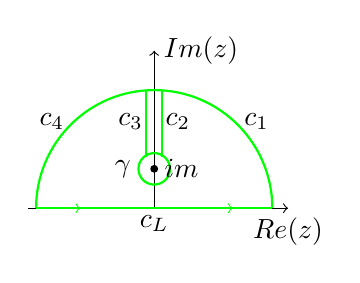
\begin{tikzpicture}

      % Linea orizzontale (asse x)
       \draw[->] (-1.6,0) -- (1.7,0)node[anchor=north]{$\mathfrak{Re} (z)$};
       \draw[->] (0,0) -- (0,2)node[anchor=west]{$\mathfrak{Im} (z)$};

        % Semicirconferenza
        \draw[thick,green] (1.5,0) arc (0:180:1.5);
        \draw[>->,green] (-1,0) -- (1,0);
        \draw[thick,green] (-1.5,0) -- (1.5,0);
        
        \node at (1.3,1.1) {$c_1$};
        \node at (-1.3,1.1) {$c_4$};
        \node at (.3,1.1) {$c_2$};
        \node at (-.3,1.1) {$c_3$};
        \node at (-.4,.5) {$\gamma$};
        \node at (0,-.2) {$c_L$};

        % Circonferenza più piccola
        \draw[thick,green] (0,0.5)node[black,anchor=west]{$im$} circle (.2);
        \fill (0,.5) circle (0.05);
        
        % Linee verticali (due segmenti paralleli all'asse y)
        \draw[thick, green] (-.1,.65) -- (-0.1,1.5);
        \draw[thick, green] (.1,.65) -- (0.1,1.5);
      \end{tikzpicture}
      \small Path used in the integration in the complex plane.
}
\begin{equation*}
    \oint dz\ ze^{izr}e^{-i\sqrt{z^2+m^2}t}=\biggl(\int_{c_1}+\int_{c_2}+\int_{c_3}+\int_{c_4}+\int_{\gamma}+\int_{c_L}\biggr)ze^{izr}e^{-i\sqrt{z^2+m^2}t}dz=0
\end{equation*}
The integral that we need is given by integration over $c_L$ in the limit of $c_L\rightarrow\mathbb{R}$, thus we need to evaluate all the other ones:
\begin{itemize}
    \item using the Darboux's inequality it is easy to see that the integral over $\gamma$ goes to 0 if the radius of the circumference ($\epsilon$) goes too 
    \begin{equation*}
        \bigg|\int_{\gamma}ze^{izr}e^{-i\sqrt{z^2+m^2}t}dz\bigg|\leq2\pi \epsilon\sup_{z\in\gamma}\bigg|ze^{izr}e^{-i\sqrt{z^2+m^2}t}\bigg|\leq2\pi m \epsilon^2\bigg|e^{-mr}e^{it\sqrt{2im\epsilon e^{i\theta_{\text{max}}}}}\bigg|;
    \end{equation*}
    \item for the path $c_4$ we can express the integrand as
    \begin{equation*}
        ze^{izr}e^{-i\sqrt{z^2+m^2}t}=ze^{i\mathfrak{Re}(z)r}e^{-i\mathfrak{Re}(\sqrt{z^2+m^2})t}e^{-\mathfrak{Im}(z)r}e^{\mathfrak{Im}(\sqrt{z^2+m^2})t},
    \end{equation*}
    since the $c_4$ is at the left of the branch cut $\mathfrak{Im}(\sqrt{z^2+m^2})<0$, thus the integrand vanishes for $|z|\rightarrow\infty$;
    \item for the path $c_1$ we cannot use the same approch as for $c_4$ but, since we want to show that the probability $ P(\vec x \rightarrow\vec y,t)$ for $|\vec x-\vec y|=r>ct$ in non-zero, we can assume $r\gg t$ (we fixed $c=1$), thus:
    \begin{equation*}
        e^{-\mathfrak{Im}(z)r}e^{\mathfrak{Im}(\sqrt{z^2+m^2})t}\approx e^{-\mathfrak{Im}(z)r}\xrightarrow{|z|\ \rightarrow \infty}\ 0;
    \end{equation*}
    \item the integrals over $c_2$ and $c_3$ are the only non-vanishing 
    \begin{equation*}
        \int_{c_L}ze^{izr}e^{-i\sqrt{z^2+m^2}t}dz=-\biggl(\int_{c_2}+\int_{c_3}\biggr)ze^{izr}e^{-i\sqrt{z^2+m^2}t}dz=-2\int_{m}^{L} ye^{-yr}\sinh(\sqrt{y^2-m^2})dy
    \end{equation*} 
\end{itemize}
In the limit $c_L\rightarrow\mathbb{R}$ we can now use these results to get:
\begin{equation*}
    P(\vec x \rightarrow\vec y,t)\xrightarrow{|\vec x-\vec y|\gg ct}\bigg|\frac{2i}{(2\pi)^2r}\int_{m}^{+\infty} ye^{-yr}\sinh(\sqrt{y^2-m^2})dy\bigg|^2\neq 0.
\end{equation*}
To make more evident that this probability is non-vanishing we can use that for $t>0$:
\begin{align*}
    &\sinh(\sqrt{y^2-m^2})<e^{\sqrt{y^2-m^2}}<e^yt\\&\Rightarrow\qquad \frac{2i}{(2\pi)^2r}\int_{m}^{+\infty} ye^{-yr}\sinh(\sqrt{y^2-m^2})dy<\frac{2i}{(2\pi)^2r}\int_{m}^{+\infty} ye^{-y(r-t)}dy\\&\qquad\qquad\qquad\qquad\qquad\qquad\qquad\qquad=\frac{2i}{(2\pi)^2r}\frac{m(r-t)+1}{(r-t)^2}e^{m(r-t)}\neq0.
\end{align*}
\section{Quantum field theory framework}
The main idea behind quantum field theory is that each fundamental particle has its own associated quantum field (such as photons and the electromagnetic field). Those particles arise as quanta of excitations of their respective fields around the ground state or vacuum.\\This approach ensures:
\begin{itemize}
    \item \textbf{Locality}: all interactions are local;
    \item \textbf{Causality}: nothing can escape the light cone;
    \item \textbf{Particle/antiparticle annihilation and creation};
    \item \textbf{Identical particle}: all particle of the same field are identical;
    \item \textbf{Bosons and Fermions}: symmetry or antisymmetry of the wave function of a particle is not imposed as in classical quantum mechanics.
\end{itemize}
In order to describe our systems as fields we will promote the fields themselves to operators acting on a so-called \textbf{Fock's space}\index{Fock's space}. Then we will have to impose commutation relations in order to quantize the system.
\subsection{Units and scales}
Before introducing the first models of quantum field theory, we will discuss the relations between the units that we will use and the scales of energy of the universe, to understand where we will be able to apply this theory.\\
The three main physical constants of nature are: the \textbf{speed of light}, the \textbf{Planck's constant} and the \textbf{Newton's constant}.
\begin{align*}
    &&[c]=\frac{L}{T},\ &&[\hslash]=M\frac{L^2}{T},\ &&[G]=\frac{L^3}{MT}.&&
\end{align*} 
From now on we will use the so-called \textbf{natural units}: $c=\hslash=1$.
\begin{align*}
    \Rightarrow&&[c]=[\hslash]=1,\ &&[G]=\frac{1}{M^2}.&&
\end{align*}
In this system everything has dimensions of a power of mass unit, we define the notation of \emph{mass-dimension} as:
\begin{equation*}
    [x]=d \quad\Rightarrow\quad [x]=M^d,\qquad\text{thus}\qquad [c]=[\hslash]=0,\ [G]=-2,\ [\lambda_C]=-1.
\end{equation*}
Lastly we define the \textbf{Planck mass} $M_P$ and \textbf{Planck length} $l_P$:
\begin{equation*}
    M_P=G^{-\frac{1}{2}}\backsimeq 10^{19}\text{Gev},\qquad l_P=M_P^{-1}\backsimeq 10^{-35}\text{m}.
\end{equation*}
The Planck mass defines the upper limit for which gravity is predominant over the other interactions. At lower energies ($M_{GUT}\backsimeq 10^{16}$GeV) we reach the point where electromagnetism, the weak and the strong interactions exists as independent interactions, exiting the \textbf{grand unified theories} energy scales. From $10^3$ Gev (energy used in \textbf{LHC}) to $0.5$ Mev we have the energy scale of the \textbf{standard model of particles}. At around $1$ meV we find the energy of a neutrino and the energy associated to the \textbf{cosmological constant}. Lastly we have the energy associated to the \text{Hubble constant}, or associated to the size of the universe ($10^{26}m$), which is $10^{-32}$ eV.\\
To have in mind this scale can help us to remember the energies for which we have tested the theoretical framework that we are going to build and for which it can hold.
\section{The mechanical model of a quantum field}
In this section we will build, from classical mechanics, a model of a field and then we will proceed to quantize it. In this way we will reproduce the steps needed to build a quantum field but always having in mind the classical meaning of it.\\
\marginnote{
    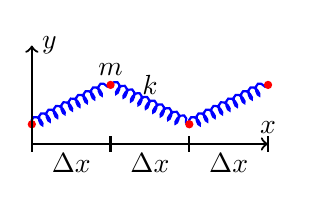
\begin{tikzpicture}[scale=.5]
        % Definizione della distanza delta
        \def\delta{1.5}
      
        
        
        % Linee e molle
        \draw[blue, thick,decorate,decoration={coil, segment length=3pt, amplitude=2pt}] (0,0.5) -- (2,1.5);
        \draw[blue, thick, decorate, decoration={coil, segment length=3pt, amplitude=2pt}] (2,1.5) --node[black,above]{$k$} (4,0.5);
        \draw[blue, thick,decorate ,decoration={coil, segment length=3pt, amplitude=2pt}] (4,0.5) -- (6,1.5);

        % Punti rossi
        \foreach \x/\y in {0/0.5, 2/1.5, 4/0.5, 6/1.5} {
          \fill[red] (\x,\y) circle (3pt);
          \draw[black,thick] (\x,-0.2) -- (\x,0.2);
        }
        
        % Etichetta delta
        \node[below] at (1, 0) {$\Delta x$};
        \node[below] at (3, 0) {$\Delta x$};
        \node[below] at (5, 0) {$\Delta x$};
        \node[above] at (2, 1.5) {$m$};

        \draw[thick,->] (0,0) -- (6,0)node[above]{$x$};
        \draw[thick,->] (0,0) -- (0,2.5)node[right]{$y$};
      \end{tikzpicture}
      \small Representation of the system of $N$ coupled oscillators.
}
The model we are going to study is the mechanical model of a string. First of all we will consider it as $N$ coupled harmonic oscillators, in the form of $N$ massive identical particles, that can move only in the y direction, connected each other by springs to form a ring (in this way the last particle is connected to the first).\\
The lagrangian reads:
\begin{equation*}
    L=T-U=\sum_{i=1}^{N}\frac{m\dot y_i^2}{2}-\sum_{i=1}^{N}\frac{k}{2}\big[y_i-y_{i-1}\big]^2,
\end{equation*}
for reasons that will be clearer later, we define $v^2=\frac{k\Delta x^2}{m}$ and then we manipulate the lagrangian to get:
\begin{equation*}
    L=\frac{m}{2}\sum_{i=1}^{N}\bigg[\dot y_i^2-v^2\bigg(\frac{y_i-y_{i-1}}{\Delta x}\bigg)^2\bigg].
\end{equation*}
Using Euler-Lagrange equations \eqref{Euler-Lagrange} we get $N$ coupled second order differential equations:
\begin{equation*}
    \ddot y_i(t)=-\bigg(\frac{v}{\Delta x}\bigg)^2\big(2y_i(t)-y_{i+1}(t)-y_{i-1}(t)\big).
\end{equation*}
In order to decouple these equations, since we are assuming periodic conditions on this system, we will perform a \emph{discrete Fourier Transform}: 
\begin{align*}
    y_j(t)&=\frac{1}{\sqrt{N}}\sum_{s=0}^{N}e^{i\frac{2\pi}{N}sj} \tilde{y}_s(t),\\
    \ddot y_j(t)&=\frac{1}{\sqrt{N}}\sum_{s=0}^{N}e^{i\frac{2\pi}{N}sj} \ddot{\tilde{y}}_s(t)\\&=-\bigg(\frac{v}{\Delta x}\bigg)^2\frac{1}{\sqrt{N}}\sum_{s=0}^{N}e^{i\frac{2\pi}{N}sj}\big(2\tilde y_s(t)-e^{i\frac{2\pi}{N}s}\tilde y_{s}(t)-e^{-i\frac{2\pi}{N}s}\tilde y_{s}(t)\big)\\&=-\bigg(\frac{v}{\Delta x}\bigg)^2\frac{1}{\sqrt{N}}\sum_{s=0}^{N}e^{i\frac{2\pi}{N}sj}\big(2-e^{i\frac{2\pi}{N}s}-e^{-i\frac{2\pi}{N}s}\big)\tilde y_{s}(t)\\&=-\bigg(\frac{v}{\Delta x}\bigg)^2\frac{2}{\sqrt{N}}\sum_{s=0}^{N}e^{i\frac{2\pi}{N}sj}\bigg(1-\cos\bigg(\frac{2\pi s}{N}\bigg)\bigg)\tilde y_{s}(t)\\&=-\frac{1}{\sqrt{N}}\sum_{s=0}^{N}e^{i\frac{2\pi}{N}sj}\bigg(\frac{2v}{\Delta x}\sin\bigg(\frac{\pi s}{N}\bigg)\bigg)^2\tilde y_{s}(t).
\end{align*}
In this way we have obtained $N$ decoupled harmonic oscillators:
\begin{equation*}
    \ddot{\tilde{y}}_s(t)=-\bigg(\frac{2v}{\Delta x}\sin\bigg(\frac{\pi s}{N}\bigg)\bigg)^2\tilde y_{s}(t)\quad\Rightarrow\quad \tilde{y}_s(t)=A_s e^{-i\omega_st},\quad\omega_s=\frac{2v}{\Delta x}\sin\bigg(\frac{\pi s}{N}\bigg).
\end{equation*}
Using again the Fourier transform we now can get an explicit solution:
\begin{equation*}
    y_j(t)=\frac{1}{\sqrt{N}}\sum_{s=0}^{N}e^{i\frac{2\pi}{N}sj}A_s e^{-i\omega_st}=\frac{1}{\sqrt{N}}\sum_{s=0}^{N}A_s e^{i\frac{2\pi}{N}sj-i\omega_st},\quad\omega_s=\frac{2v}{\Delta x}\sin\bigg(\frac{\pi s}{N}\bigg),
\end{equation*}
this is the superposition of $N$ harmonic waves each with its own waves number and velocity:
\begin{equation*}
    k_s=\frac{2\pi s }{N\Delta x},\quad v_s=\frac{\omega_s}{k_s}=v\sin\bigg(\frac{\pi s}{N}\bigg)\frac{N}{\pi s}.
\end{equation*}
We should now notice that this model allows only $\frac{N}{2}-1$ independent oscillators: the last oscillator has $\omega_s=0$, for $s=\frac{N}{2}$ $\omega_s$ is maximum and for $s>\frac{N}{2}$ all the $\omega_s$ are the same of those with $s<\frac{N}{2}$ (since the sine function is symmetric in the interval $[0,\pi]$).\\Due to the fact that the equation of motion must be real, we can see that:
\begin{align*}
    y_j(t)&=\frac{1}{\sqrt{N}}\sum_{s=0}^{\frac{N}{2}-1}e^{i\frac{2\pi}{N}sj} \tilde{y}_s(t)+\frac{1}{\sqrt{N}}\sum_{s=\frac{N}{2}+1}^{N}e^{i\frac{2\pi}{N}sj} \tilde{y}_s(t)+\tilde{y}_\frac{N}{2}(t)+\tilde{y}_N(t)\\&=\frac{1}{\sqrt{N}}\sum_{s=0}^{\frac{N}{2}-1}\bigg[ e^{i\frac{2\pi}{N}sj} \tilde{y}_s(t)+e^{i\frac{2\pi}{N}j(N-s)} \tilde{y}_{N-s}(t)\bigg]
   +\tilde{y}_\frac{N}{2}(t)+\tilde{y}_N(t)\\&=\frac{1}{\sqrt{N}}\sum_{s=0}^{\frac{N}{2}-1}\bigg[ e^{i\frac{2\pi}{N}sj} \tilde{y}_s(t)+e^{-i\frac{2\pi}{N}js} \tilde{y}_{N-s}(t)\bigg]
   +\tilde{y}_\frac{N}{2}(t)+\tilde{y}_N(t)\\&=y_j^*=\frac{1}{\sqrt{N}}\sum_{s=0}^{\frac{N}{2}-1}\bigg[ e^{-\frac{2\pi}{N}sj} \tilde{y}^*_s(t)+e^{i\frac{2\pi}{N}js} \tilde{y}^*_{N-s}(t)\bigg]
   +\tilde{y}^*_\frac{N}{2}(t)+\tilde{y}^*_N(t)\\
   &\Rightarrow\qquad \tilde y_s=\tilde y_{N-s}^*,\qquad \tilde y_s^*=\tilde y_{N-s}, \quad \forall s\neq\frac{N}{2},N.
\end{align*}
This decoupling process can be used to diagonalize the lagrangian, which reads:
\begin{equation*}
    L=m\sum_{s=1}^{\frac{N}{2}-1}\bigg[|\dot{\tilde{y}}_s|^2-\omega_s^2|\tilde{y}_s|^2\bigg].
\end{equation*}

We will now proceed to quantize this simple system. In order to do so we remind that the simple quantum oscillator, with an hamiltonian operator
\begin{equation*}
    \hat{\mathcal{H}}=\frac{\hat{ P^2}}{2m}+\frac{\omega^2}{2}\hat{ y^2}, 
\end{equation*}
can be quantized introducing the \textbf{creation/annihilation operators}:
\begin{align*}
    &\hat{ a}=\sqrt{\frac{\omega}{2}}\hat{y} +\frac{i}{\sqrt{2\omega}}\hat{ P},\qquad &\hat{a}^\dagger=\sqrt{\frac{\omega}{2}}\hat{ y} -\frac{i}{\sqrt{2\omega}}\hat{ P},\\ &[\hat{a},\hat{ a}^\dagger ]=\hat{\mathds{1}},\qquad &[\hat{\mathcal{H}},\hat{ a}^\dagger ]=\omega\hat{ a}^\dagger,\\
    &\hat{ \mathcal{H}} =\omega\bigg(\hat{N}+\frac{1}{2}\bigg),&\hat N=\hat{ a}^\dagger\hat{ a}.
\end{align*}
Every eigenstate of the hamiltonian is created using the $\hat a^\dagger$ operator: given the ground state $\ket{0}$ it easy to deduce that:
\begin{equation*}
    \hat{\mathcal{H}} \big(\hat{a}^\dagger \big)^n\ket{0}=(E_n+\omega)\big(\hat{a}^\dagger\big)^n\ket{0},\quad \Rightarrow\quad \big(\hat{a}^\dagger \big)^n\ket{0}=\sqrt{n!}\ket{n}.
\end{equation*}
In order to quantize our system we will promote every $\tilde y_i$ to an operator:
\begin{equation*}
        \hat{\mathfrak{Re}\tilde{y} }_s=\frac{\hat{a}^{(R)}_{s}+\hat{a}^{(R)\dagger}_{s}}{\sqrt{2\omega_s}},\qquad
        \hat{\mathfrak{Im} \tilde{y} }_s=\frac{\hat{a}^{(I)}_{s}+\hat{a}^{(I)\dagger}_{s}}{\sqrt{2\omega_s}},\qquad s\in[1,N/2]\cap\mathbb{N}. 
\end{equation*} 
In this way each harmonic oscillator will have its own Hilbert space $\mathcal{H}_{\omega_s}$, the whole system will be described by a more complicated combination of these Hilbert spaces. We than define the Hilbert space $\mathcal{H}_k=\otimes_{s=1}^k \mathcal{H}_{\omega_s}$, a generic state is now described in a Fock Space $\mathcal{F} =\oplus_{i=1}^{N} \mathcal{H}_i$. The state of the system will be a linear combination of vectors in the form:
\begin{equation*}
    \big(\hat{a}^{(R)\dagger}_{i_1}\big)^{n_1^R}\big(\hat{a}^{(R)\dagger}_{i_2^R}\big)^{n_2}\dots \big(\hat{a}^{(I)\dagger}_{i_1}\big)^{n_1^I}\big(\hat{a}^{(I)\dagger}_{i_2}\big)^{n_2^I}\dots\ket{0}=\ket{n_i^R,n_2^R,\dots,n_i^I,n_2^I,\dots},
\end{equation*}
where the vacuum state $\ket{0}$ should be intended as
\begin{equation*}
    \ket{0}=\ket{0}_{\omega_1}^R\otimes\ket{0}_{\omega_2}^R\otimes\dots\ket{0}_{\omega_1}^I\otimes\ket{0}_{\omega_2}^I\otimes\dots\ .
\end{equation*}
In this way, for example, the state of a system with $1$ particle with energy $\omega_1$ and $2$ with energy $\omega_4$ will be represented by:
\begin{equation*}
    \hat{a}^{(R)\dagger}_{\omega_1} \big(\hat{a}^{(R)\dagger}_{\omega_4}\big)^2\ket{0}=\ket{1,0,0,2,0,\dots}.
\end{equation*}
In this way the hamiltonian of the whole system becomes:
\begin{equation*}
    \hat{\mathcal{H}} = \sum_{s=1}^{\frac{N}{2}-1}\omega_s\big(\hat{ N}_s+1\big),
\end{equation*}
it is now possible to observe a non-trivial aspect of the theory that we are building, in fact the energy of the vacuum state, when there are many particles in the system, is not negligible due to the constant identity operator that appear in the hamiltonian.\\

We will now take the continuum limit, that considering $N\rightarrow\infty$ and $\Delta x\rightarrow 0$ will lead us to the generalization of the $N$ solutions of our system to a field:
\begin{equation*}
    j\Delta x\quad \xrightarrow[\Delta x\rightarrow0]{N\rightarrow\infty}\quad x,\qquad y_s(t)\quad\xrightarrow[\Delta x\rightarrow0]{N\rightarrow\infty}\quad\psi(x,t).
\end{equation*}
The mechanical properties of the string, such as the velocity of the waves, also will be affected by this limiting procedure:
\begin{equation*}
    v_s=\frac{\omega_s}{k_s}=v\sin\bigg(\frac{\pi s}{N}\bigg)\frac{N}{\pi s}\xrightarrow[\Delta x\rightarrow0]{N\rightarrow\infty}v,\quad \omega_s=2\frac{v}{\Delta x}\sin\bigg(\frac{\pi s}{N}\bigg)\xrightarrow[\Delta x\rightarrow0]{N\rightarrow\infty}vk.
\end{equation*}
Quantizing this system we can obtain phonons which obey some sort of "relativistic massless energy" (considering $v=c$):
\begin{equation*}
    \omega_k=cK\quad\Rightarrow\quad  \hslash\omega_k=\hslash cK\quad\Rightarrow\quad E_p=pc,
\end{equation*}
in this way we could interpret this filed, that arises from the string model, as a relativistic massless particle.\\

Modifying the initial discrete lagrangian, we could add a term to introduce mass. This term can be introduced by inserting a new elastic interaction which attracts every point mass to its own equilibrium point, independently of the others masses.
\marginnote{
    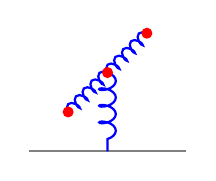
\begin{tikzpicture}[scale=0.5]
        % Definizione delle coordinate dei punti
        \coordinate (A) at (0,0);
        \coordinate (B) at (1,1);
        \coordinate (C) at (2,2);
        
        % Punti rossi
        
        
        % Linee e molle tra i punti
        \draw[blue, thick, decorate, decoration={coil, segment length=4pt, amplitude=2pt}] (A) -- (B);
        \draw[blue, thick, decorate, decoration={coil, segment length=4pt, amplitude=2pt}] (B) -- (C);
        
        % Linea grigia orizzontale
        \draw[gray, thick] (-1,-1) -- (3,-1);
        
        % Molla verticale verde
        \draw[blue, thick, decorate, decoration={coil, segment length=6pt, amplitude=3pt}] (B) -- (1,-1);
        \foreach \point in {A,B,C} {
          \fill[red] (\point) circle (4pt);
        }
      \end{tikzpicture}\\
      \small A sketch of the system with the interaction needed to consider massive particles.
}
\begin{equation*}
    L=\sum_{i=1}^{N}\bigg[\frac{m}{2}\dot y_i^2-\frac{m}{2}v^2\bigg(\frac{y_i-y_{i-1}}{\Delta x}\bigg)^2-\frac{K_\mu}{2} y_j^2\bigg].
\end{equation*}
To end this introduction we will study the continuum limit of this modified largrangian. The sum over all the point masses becomes an integral over the length of the string:
\begin{equation*}
    L=\int dx\bigg[\frac{m}{2}\bigg(\frac{\partial\psi}{\partial t}\bigg)^2-\frac{m}{2}v^2\bigg(\frac{\partial\psi}{\partial x}\bigg)^2-\frac{K_\mu}{2}\psi^2\bigg].
\end{equation*} 
The integrand we have obtained is a \textbf{lagrangian density} and we will see that this will become the object describing the proprieties of the fields. This particular one is the lagrangian density of the \textbf{Klein-Gordon field}, which, as we supposed, describes massive relativistic spin zero particles. By the Euler-Lagrange equations this lagrangian density gives as equations of motion the Klein-Gordon equation :
\begin{equation*}
    m\partial_\mu\partial^\mu\psi+K_\mu\psi=0.
\end{equation*}
Again this is a series of infinitely many coupled harmonic oscillators that can be decoupled by the Fourier Transform: each one of these will have a relativistic energy of a massive particle with a precise momentum.

